\subsection{User Study}
To further evaluate the effectiveness of $\avats$ from the the audience perspective, we conducted formal user studies to compare how users perform the urban exploration tasks with visualizations generated by whole dataset, \textit{random sampling} and $\avats$.


\begin{figure}[t]
	\centering
	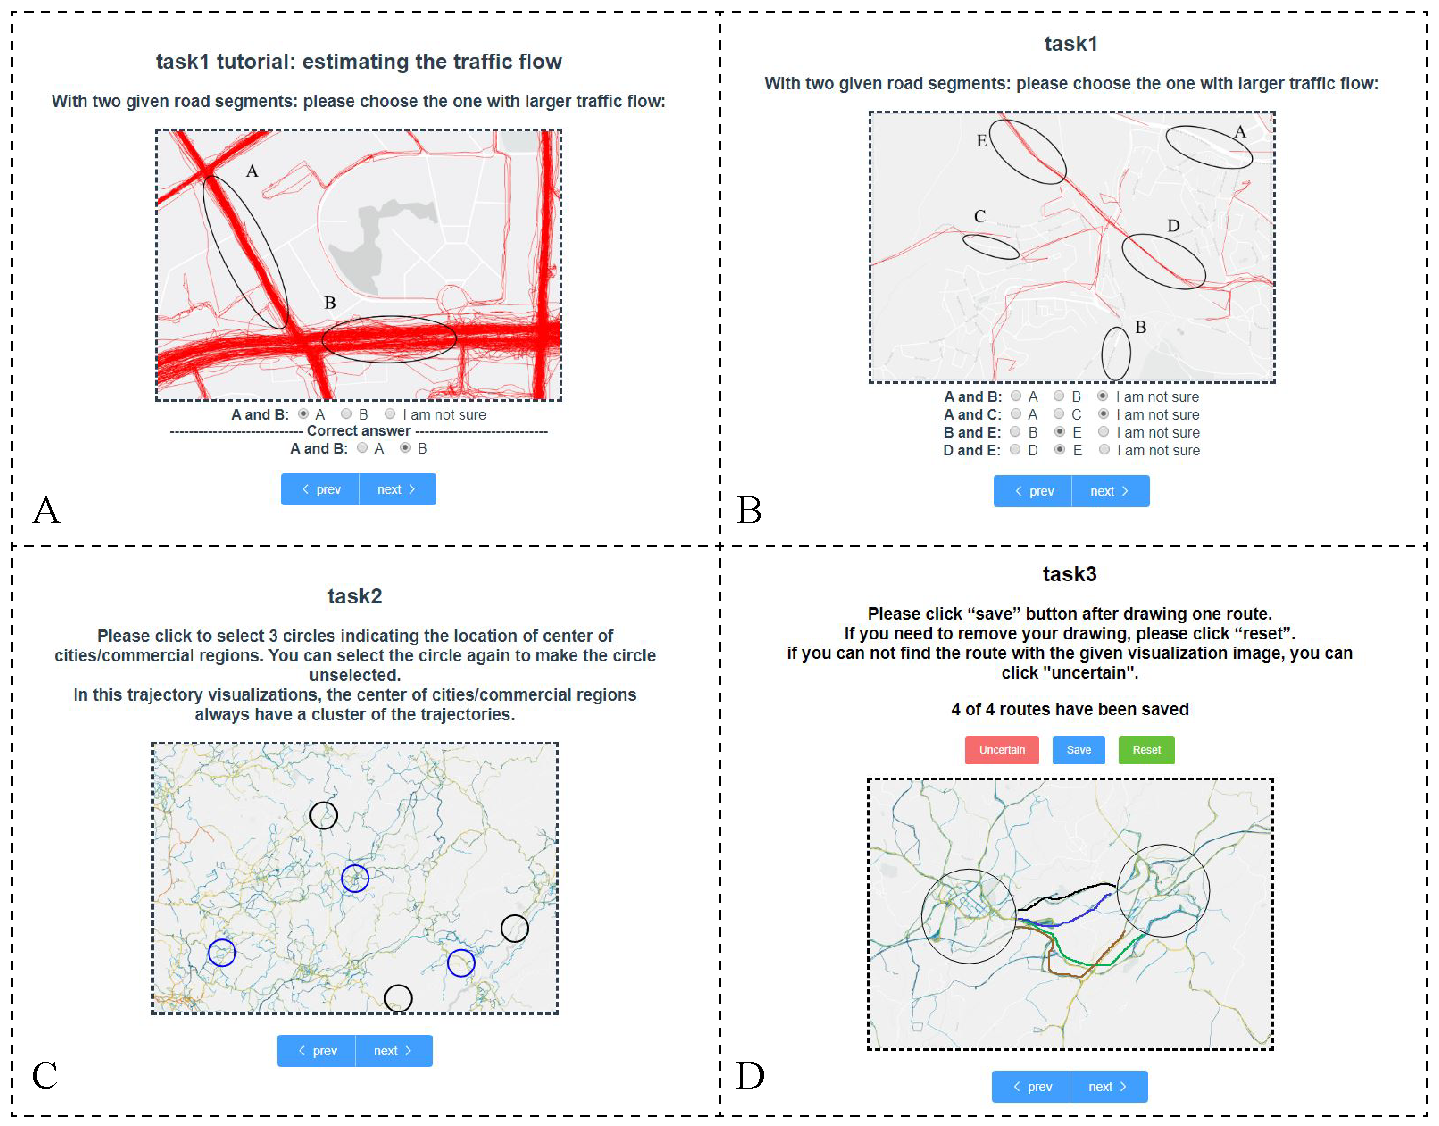
\includegraphics[width=0.48\textwidth]{pictures/user_study/interface.pdf}
	\vspace{-3mm}
	\caption{The interface of user study platform.}
	\vspace{-5mm}
	\label{fig:user_study}
\end{figure}

\subsubsection{Experiment setting}

\stitle{Participants and apparatus}
We recruit 100 participants (** females, ** males, aged 20 to **(mean=**, SD=**)) with normal vision or normal corrected vision. All of these participants have the background of computer science. 
The study system is a web-based platform which has the size-fixed interface and the participants perform the user study on their own  computers. The system interface is shown as Figure~\ref{fig:user_study}. Considering the unfairness caused by the screen size, we recommend all participants to set the resolution of the screen as 1980 * 1080 before the experiment. All images displayed on the interface have the same size of(AA*BB).  

\stitle{Tasks and data generation}
We used the taxi trajectory dataset of Porto and Shenzhen for the user study. All participants needed to perform three types of tasks: \textbf{traffic flow estimation},\textbf{ city/commercial region center identification} and Reachable route inspection(shown as Figure~\ref{fig:user_study}(B,C,D)). For all the tasks, we have generated 145 visualizations(35 for T1, 75 for T2, 35 for T3) and 185 different questions(12 for T1, 152 for T2, 21 for T3). 

\textbf{T1. Traffic flow estimation}. 
% what participants do
As shown by Figure~\ref{fig:user_study}(B), with a given visualization, some road segments will be identified by ellipses(shown as~\ref{fig:user_study}(B)). Several road segment pairs were randomly selected and listed below the view. The participants were asked to choose the one with larger traffic flow by clicking the radio box. They can also choose ``I am not sure'' if they cannot decided the answer. 
%Why possible
A road with larger traffic flow has more trajectories in the dataset passing through the road segment, thus lead to a denser and broader trajectory brunch in the visualization. In the trajectory visualization with color encoding, such kind of pattern can also be highlighted by a concentration of trajectories with warm color. 
%Generate the data
To generate the test data of T1,  we sampled and selected the visualization views which contain clear road structures. Then the number of trajectories passing through each road segment was counted as the traffic flow. 

\textbf{T2. City/commercial region center identification.} 
% what participants do
As shown by Fig

ure~\ref{fig:user_study}(C), a visualization view was given and several regions were marked by circle. The participants needed to select the regions which could be city/commercial centers by click the corresponding circles. In each task, the number of correct regions were given. 
%Why possible
The city or commercial region centers always have more passing trajectories from different directions than the surrounding regions, which results in the \UC{start-shape} cluster of trajectories in the visualization. 
%Generate the data
To generate the test data of T2, we randomly chose several visualization views which contain city/commercial regions and labeled the locations of each city/commercial region center on the visualization as the correct locations first.  Then we randomly generated locations and remove the locations close to the correct locations, the remaining locations are the error locations. In each task of T2, with a given visualization, the same number of correct and wrong locations will be randomly selected. 

\textbf{T3. Reachable route inspection.} 
% what participants do
Figure~\ref{fig:user_study}(D) shows the interface of T3, which includes a visualization and two circular regions. The users needed to draw several most representative reachable routes to connect the two regions. The number of the reachable routes is given. 
%Why possible
The reachable routes indicate the routes connecting two regions, these routes must have the passing trajectories. 
%Generate the data
To generate the test data, we randomly chose the visualization views which contain two or more city/commercial regions. In each task of T2, a visualization and two regions were randomly selected.


\stitle{Procedure}
The user study began with the introduction which introduces the motivation, tasks and visual encoding. Then the following sessions are divided into three blocks according to the task types. Each block starts with a task tutorial, in which the participants could perform several demo tasks, thus familiarizing themselves with the interface, interaction and tasks. For example, Figure~\ref{fig:user_study}(A) shows the demo task of T1, in which the users can check the correct answer after clicking the ``check'' button. After all the questions are finished, the answers and time usage are collected and saved in the database for the further analysis. At last, a post-interview were conducted to collect the feedback of the participants.  


\subsubsection{Results}
Figure~\ref{fig:accuracy} depicts the accuracy among the task types and sampling methods. With a given task type and method, we visualize the average accuracy by a colored circle and a line-segment to indicate the highest and lowest score if each question. 

\begin{figure}[t]
	\centering
	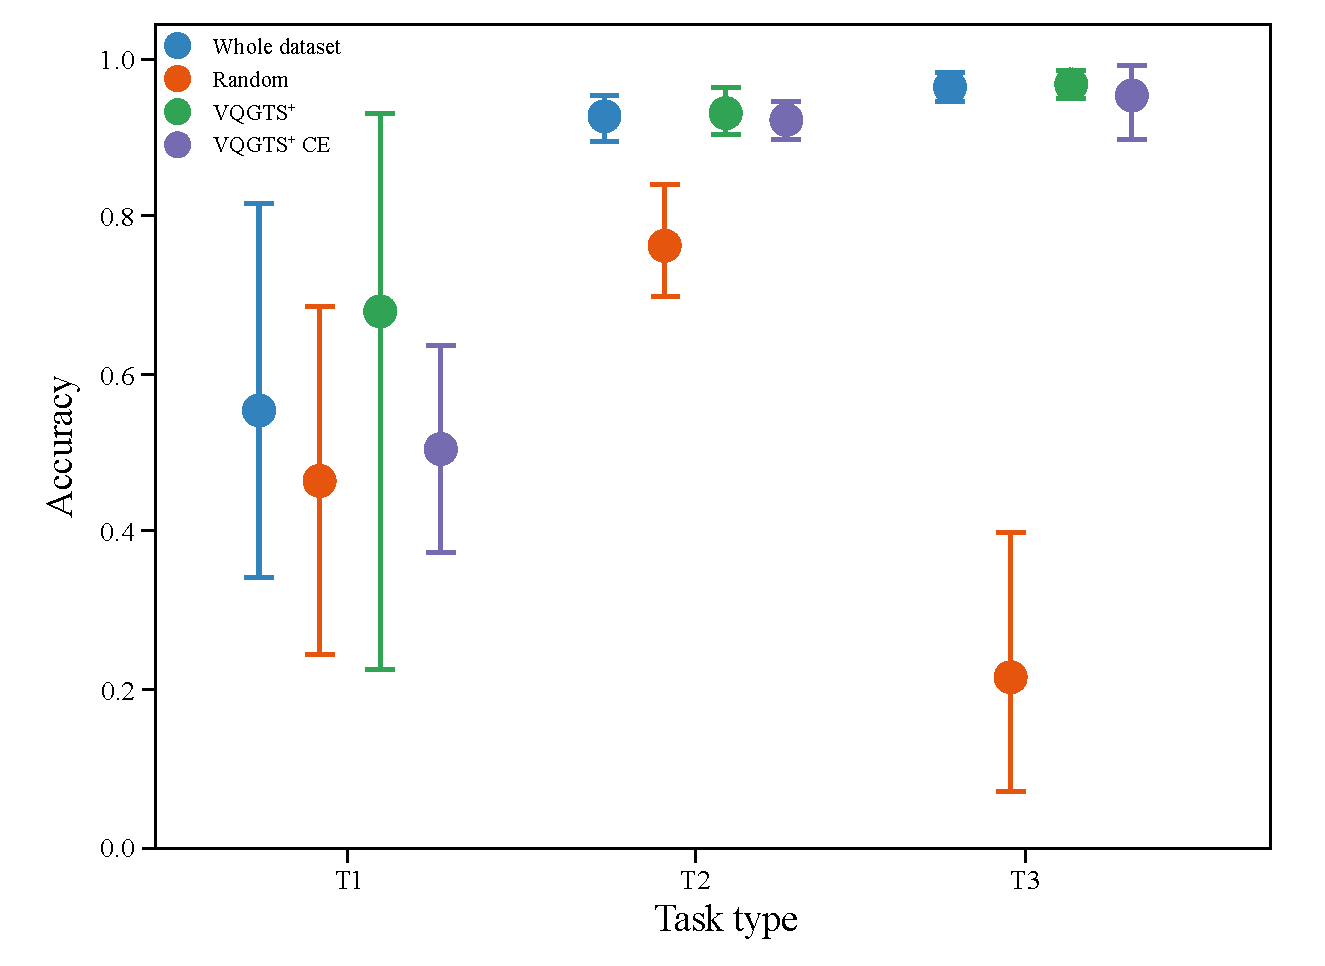
\includegraphics[width=0.44\textwidth]{pictures/user_study/accuracy.pdf}
	\vspace{-3mm}
	\caption{Average accuracy of three types of tasks. X axis indicates the task types and methods. Y axis indicate the accuracy.}
	\vspace{-5mm}
	\label{fig:accuracy}
\end{figure}

\stitle{Accuracy} 
Figure~\ref{fig:accuracy} summarizes the accuracy of all the tests. We observe that the $\avats$ and whole dataset outperform the random method in all these three types of tasks. The accuracy distribution based on whole dataset, $\avats$ and $\avats$ with color encoding are close to each other, indicating the proposed approach can replace the whole dataset when performing these three tasks. 



\stitle{Time usage}

\stitle{Post interview}